\documentclass[man]{apa6}
\usepackage{lmodern}
\usepackage{amssymb,amsmath}
\usepackage{ifxetex,ifluatex}
\usepackage{fixltx2e} % provides \textsubscript
\ifnum 0\ifxetex 1\fi\ifluatex 1\fi=0 % if pdftex
  \usepackage[T1]{fontenc}
  \usepackage[utf8]{inputenc}
\else % if luatex or xelatex
  \ifxetex
    \usepackage{mathspec}
  \else
    \usepackage{fontspec}
  \fi
  \defaultfontfeatures{Ligatures=TeX,Scale=MatchLowercase}
\fi
% use upquote if available, for straight quotes in verbatim environments
\IfFileExists{upquote.sty}{\usepackage{upquote}}{}
% use microtype if available
\IfFileExists{microtype.sty}{%
\usepackage{microtype}
\UseMicrotypeSet[protrusion]{basicmath} % disable protrusion for tt fonts
}{}
\usepackage{hyperref}
\hypersetup{unicode=true,
            pdftitle={Reproducing: The Sound of Intellect: Speech Reveals a Thoughtful Mind, Increasing a Job Candidate's Appeal},
            pdfauthor={Troy Funderburk},
            pdfkeywords={communication, voice, speech, mind perception, social cognition,
decision making, open data},
            pdfborder={0 0 0},
            breaklinks=true}
\urlstyle{same}  % don't use monospace font for urls
\usepackage{graphicx,grffile}
\makeatletter
\def\maxwidth{\ifdim\Gin@nat@width>\linewidth\linewidth\else\Gin@nat@width\fi}
\def\maxheight{\ifdim\Gin@nat@height>\textheight\textheight\else\Gin@nat@height\fi}
\makeatother
% Scale images if necessary, so that they will not overflow the page
% margins by default, and it is still possible to overwrite the defaults
% using explicit options in \includegraphics[width, height, ...]{}
\setkeys{Gin}{width=\maxwidth,height=\maxheight,keepaspectratio}
\IfFileExists{parskip.sty}{%
\usepackage{parskip}
}{% else
\setlength{\parindent}{0pt}
\setlength{\parskip}{6pt plus 2pt minus 1pt}
}
\setlength{\emergencystretch}{3em}  % prevent overfull lines
\providecommand{\tightlist}{%
  \setlength{\itemsep}{0pt}\setlength{\parskip}{0pt}}
\setcounter{secnumdepth}{0}
% Redefines (sub)paragraphs to behave more like sections
\ifx\paragraph\undefined\else
\let\oldparagraph\paragraph
\renewcommand{\paragraph}[1]{\oldparagraph{#1}\mbox{}}
\fi
\ifx\subparagraph\undefined\else
\let\oldsubparagraph\subparagraph
\renewcommand{\subparagraph}[1]{\oldsubparagraph{#1}\mbox{}}
\fi

%%% Use protect on footnotes to avoid problems with footnotes in titles
\let\rmarkdownfootnote\footnote%
\def\footnote{\protect\rmarkdownfootnote}


  \title{Reproducing: The Sound of Intellect: Speech Reveals a Thoughtful Mind,
Increasing a Job Candidate's Appeal}
    \author{Troy Funderburk\textsuperscript{1}}
    \date{}
  
\shorttitle{MidTerm Reproduction}
\affiliation{
\vspace{0.5cm}
\textsuperscript{1} Brooklyn College}
\keywords{communication, voice, speech, mind perception, social cognition, decision making, open data\newline\indent Word count: X}
\usepackage{csquotes}
\usepackage{upgreek}
\captionsetup{font=singlespacing,justification=justified}

\usepackage{longtable}
\usepackage{lscape}
\usepackage{multirow}
\usepackage{tabularx}
\usepackage[flushleft]{threeparttable}
\usepackage{threeparttablex}

\newenvironment{lltable}{\begin{landscape}\begin{center}\begin{ThreePartTable}}{\end{ThreePartTable}\end{center}\end{landscape}}

\makeatletter
\newcommand\LastLTentrywidth{1em}
\newlength\longtablewidth
\setlength{\longtablewidth}{1in}
\newcommand{\getlongtablewidth}{\begingroup \ifcsname LT@\roman{LT@tables}\endcsname \global\longtablewidth=0pt \renewcommand{\LT@entry}[2]{\global\advance\longtablewidth by ##2\relax\gdef\LastLTentrywidth{##2}}\@nameuse{LT@\roman{LT@tables}} \fi \endgroup}


\DeclareDelayedFloatFlavor{ThreePartTable}{table}
\DeclareDelayedFloatFlavor{lltable}{table}
\DeclareDelayedFloatFlavor*{longtable}{table}
\makeatletter
\renewcommand{\efloat@iwrite}[1]{\immediate\expandafter\protected@write\csname efloat@post#1\endcsname{}}
\makeatother
\usepackage{lineno}

\linenumbers

\authornote{

Correspondence concerning this article should be addressed to Troy
Funderburk, 17 Lackawanna Pl, Bloomfield, NJ 07003. E-mail:
\href{mailto:troyfunderburk2@gmail.com}{\nolinkurl{troyfunderburk2@gmail.com}}}

\abstract{
A persons intellect can be measured in many ways. What is the difference
of intellect observation from written to spoken elevator pitches?

The research suggests that a persons verbal cues will present a higher
level of intellect than that of a written pitch.

As a result the study found that evaluators rated a candidate as more
competent, thoughtful, and intelligent when they heard a pitch rather
than read it and, as a result, had a more favorable impression of the
candidate and were more interested in hiring the candidate.


}

\begin{document}
\maketitle

\section{Methods}\label{methods}

\subsection{Participants}\label{participants}

Thirty-nine professional recruiters (mean age = 30.85 years, SD = 6.24;
9 males) from Fortune 500 companies voluntarily agreed to evaluate
pitches of job candidates from the University of Chicago Booth School of
Business.

\subsection{Material}\label{material}

Recordings of elevator pitches from three job candidates. A computerized
survey including a likert scale response.

\subsection{Procedure}\label{procedure}

Randomly selected three job candidates' spoken pitches. In an online
survey, they randomly assigned recruiters to either listen to one of the
spoken pitches (audio condition) or read the transcription of one of
those pitches (transcript condition). They recorded how long each
recruiter spent on the survey page with the stimulus. The recruiters
then answered the same survey items as a previous experiment, with one
change: All responses were recorded on Likert scales labeled from 0 to
10. Recruiters then completed a memory test in which they reported
\enquote{everything you can remember about the pitch} the MBA student
gave.

\subsection{Data analysis}\label{data-analysis}

\section{Results}\label{results}

There was a statistical significqnce for higher intellectual ratings
towards verbal over written pitches. An independent t-test releaved
written pitches (M=4.67,SD=1.97) and for verbal pitches (M=5.77,SD=.255)
conditions t(33)=2.36, p = .024.
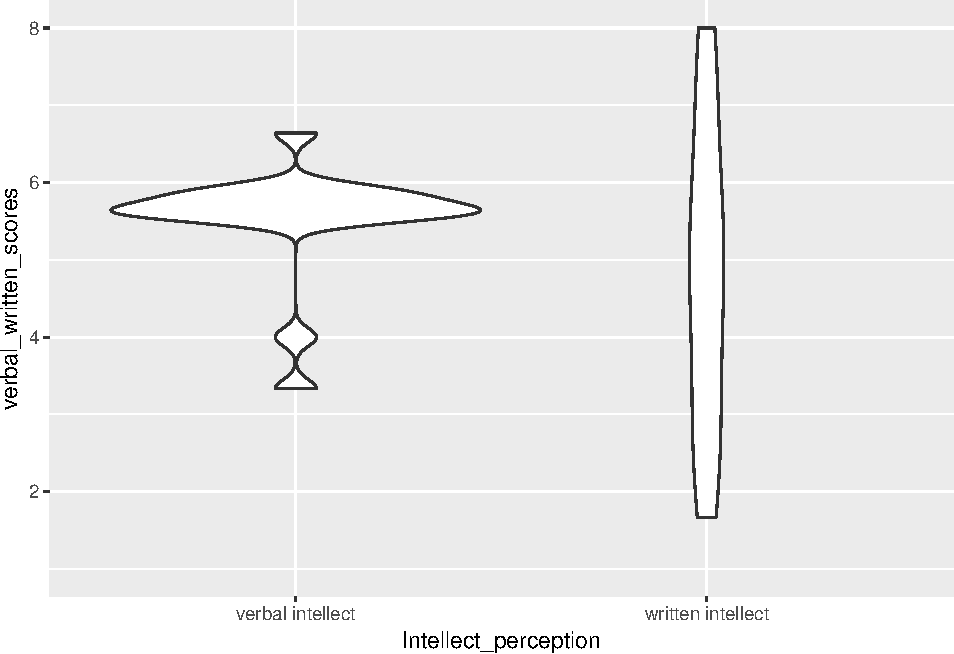
\includegraphics{Mid-Term_files/figure-latex/unnamed-chunk-1-1.pdf}

\section{Discussion}\label{discussion}

The words that come out of a person's mouth convey the presence of a
thoughtful mind more effectively than the words that are typed. Lastly,
the experiments exposed some practical implications for a necessity of
in person interaction.

\newpage

\section{References}\label{references}

RStudio Team (2015). RStudio: Integrated Development for R. RStudio,
Inc., Boston, MA URL \url{http://www.rstudio.com/}.

Schroeder, J. \& Epley, N. (2015) The sound of intellect: speech reveals
a thoughtful mind, increasing a job candidate's appeal. Psychological
Science. 26(6) 877-891.\url{doi:10.1177/0956797615572906}

\begingroup
\setlength{\parindent}{-0.5in} \setlength{\leftskip}{0.5in}

\hypertarget{refs}{}

\endgroup


\end{document}
